\chapter{Related Works}

This chapter summarises recent work on the analysis and learning of CA. We focus on the two classes of CA presented in Chapter~\ref{preliminaries}, life-like CA and Gray-Scott models.

\section{Life-Like CA: Exploration} \label{sec: life-like-exploration}

The choices of lattice geometry, neighbourhood function, state variable, and transition rule define the behaviour of a CA. Fixing the former three factors, Wolfram\cite{wolfram1986theory} classified CA based on transition rules as follows:
\begin{definition}[Wolfram Classes]\label{def:wolfram-classes} The four Wolfram classes are:
\begin{itemize}
  \item Class 1 (Null) : Rules that lead to a trivial, homogenous state
  \item Class 2 (Fixed-point / Periodic) : Rules that lead to localized stable or periodic patterns
  \item Class 3 (Chaotic) : Rules that lead to continued, unending chaos
  \item Class 4 (Complex) : Rules that can lead to complex, long-lived impermanent patterns
\end{itemize}
\end{definition}

Early attempts to categorise 2D CA by Packard and Wolfram\cite{packard1985two} extend Wolfram's original four categories. They classify rules based on information content and rate of information transmission measured using Shannon entropy and Lyapunov exponents respectively. These works provide the basis for exploration and classification of life-like CA. However, Wolfram's classes do not have clear decision boundaries and these metrics do not help quantitatively define them either. This is because Wolfram's classes are based on the characteristics that a CA is capable of possessing under \textit{some} not \textit{all} initial conditions. Equivalently, they are based on what a CA \textit{cannot} do.  For example, a class 2 CA is one which cannot exhibit chaotic patterns. This makes it impossible to classify CA before observing the result of their simulation. As proven by Yaku\cite{yaku1973constructibility}, many questions about global properties of 2D CA are formally undecidable which makes the construction of definitions based on long-term outcomes difficult and limits the usefulness of Wolfram's taxonomy.\\

Adamatzky et al.\cite{adamatzky2006phenomenology} produces a systematic analysis of life-like CA in which the birth and survival sets are contiguous intervals. These are dubbed "binary-state reaction-diffusion cellular automata (RDCA)" as they provide a discretized model of simple two-chemical reactions with substrate `0' and reagent `1'. The birth set is analogous to diffusion rate and the survival set is analogous to reaction rate. The analysis includes categorisations based on qualitative factors like the features and density of resulting configurations. It also includes quantitative factors such as the outcome of glider collisions within each universe. For example, the \textbf{P}-class contains rules with high diffusion rate (i.e. wide birth interval) and low reaction rates (i.e. narrow survival interval) which produce large regions of 0-state and 1-state each containing scatterings of the other within them. These patterns are qualitatively distinct from, for example, \textbf{O}-class rules which have low diffusion rate and high reaction rate producing irregular spotted patterns. These are shown in Figure~\ref{fig:po-class}. Despite the depth of this investigation, the 1296 CA rules analysed cover less that 0.05\% of all life-like CA. The broader issue in both Wolfram's and Adamatzky's classifications is the lack of objective distinction between class boundaries which makes it difficult to predict the behaviour of rules \textit{a priori}. Indeed, some CA have been proven to span multiple classes\cite{baldwin1999classi}.\\

\begin{figure}[!h]
\centering
            \subfloat[B12345678/S23]{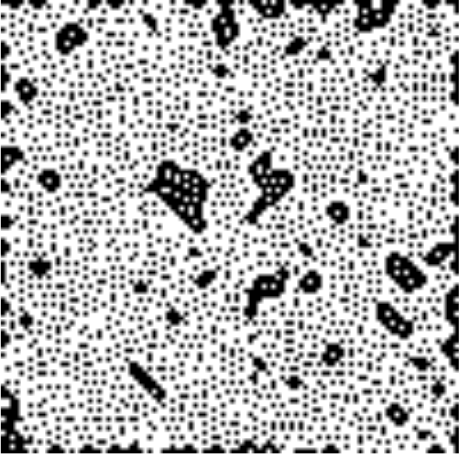
\includegraphics[width=.2\textwidth]{images/pclass1.png}}\hfill
            \subfloat[B12345678/S234]{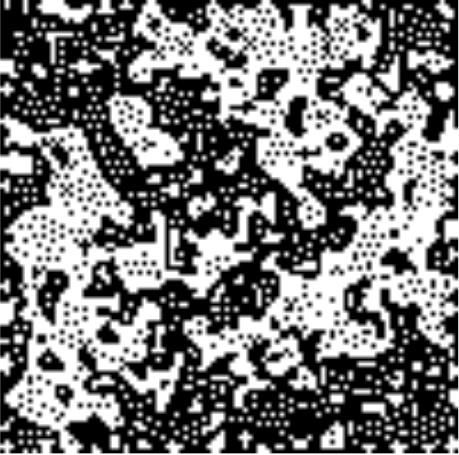
\includegraphics[width=.2\textwidth]{images/pclass2.png}}\hfill
            \subfloat[B1/S345]{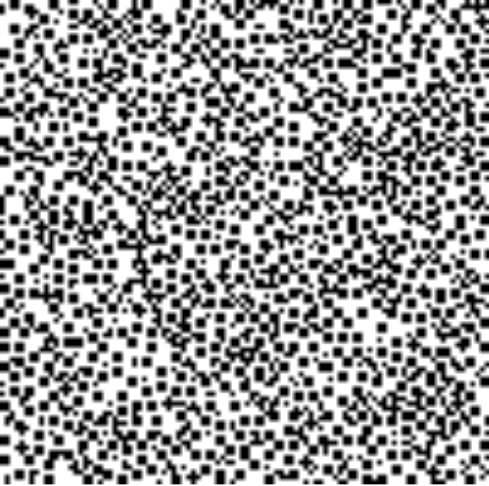
\includegraphics[width=.2\textwidth]{images/oclass1.png}}\hfill
            \subfloat[B1/S345678]{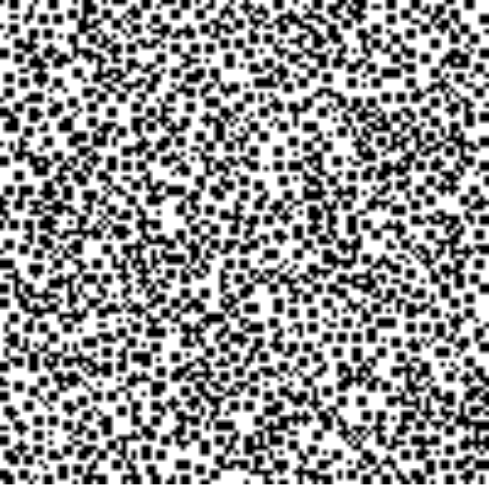
\includegraphics[width=.2\textwidth]{images/oclass2.png}}
            \caption{Configurations generated from \textbf{P}-class (a,b) and \textbf{O}-class (c,d) rules \cite{adamatzky2006phenomenology}}
\label{fig:po-class}
\end{figure}

This dilemma is alleviated to some degree by Eppstein's four-way classification\cite{eppstein2010growth} which is based on strict definitions of \textit{fertility} and \textit{mortality}. A rule is fertile if there exists a finite pattern that eventually escapes any bounding box B. Note this is symmetrically opposite to the definition of periodicity since any infertile rule can only iterate through $2^{|B|}$ steps before repeating a previous state. A rule is mortal if it supports a pattern which transitions to the \textit{quiescent} state (i.e no live cells) in the next time step. Eppstein conjectures that "interesting" behaviour arises out of rules that are both fertile and mortal. Figure~\ref{fig:eppstein-map} depicts a schematic map of his analysis.\\

\begin{figure}[!h]
\centering
    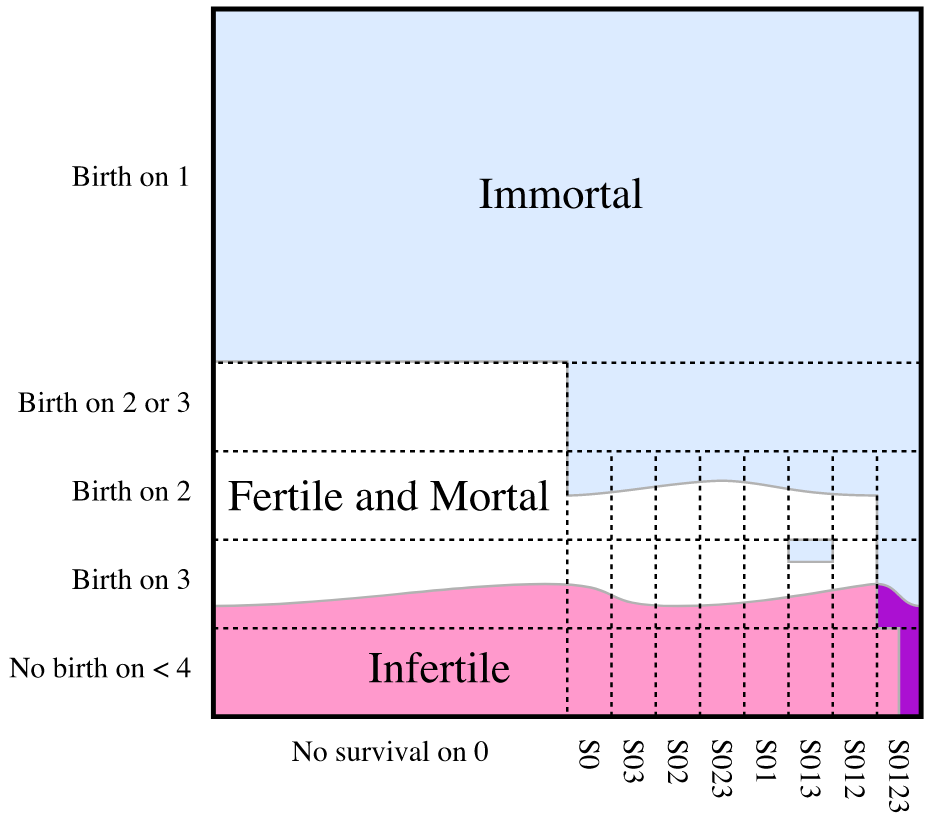
\includegraphics[width=.5\textwidth]{images/eppstein-map.png}
    \caption{Map of fertile, infertile, mortal, and immortal regions in binary-state RDCA rulespace \cite{eppstein2010growth}}
\label{fig:eppstein-map}
\end{figure}

This work provides a strong theoretical foundation to guide our search of life-like CA and to verify that our techniques are effective on different varieties. However, they are not grounded in a systematic statistical search which makes it difficult to ascertain the proportion of each category that exist in contested regions. For example, we may be interested in the ratio of fertile to infertile configurations for rule B3/S01. Although a closed-form solution for this ratio is infeasible, it is possible to come to an approximation through simulation. As mentioned in the preliminaries, large scale simulations of random initial conditions on particular rules have proven to be an effective way of identifying new patterns\cite{flammenkamp}. This is called soup searching. In a similar vein, we will use soup searches to approximate the periodicity of all rules in the life-like CA rulespace.

\section{Life-Like CA: Learning}

A seminal work by Meyer et al.\cite{meyer1989learning} looks at learning 2D CA neighbourhood functions using genetic algorithms. Later works by Mitchell et al.\cite{mitchell1996evolving} explore the effectiveness of genetic algorithms in learning entire transition functions but only in the domain of elementary cellular automata. Around the same time, Koza et al. make leaps by applying genetic programming to a broad variety of tasks including the CA majority classification problem\cite{andre1996discovery}. Incremental improvements have been made since then with Breukelaar and B{\"a}ck\cite{breukelaar2005using} delivering experimental evidence that the CA inverse design problem using evolutionary computation is more tractable in higher dimensions. We delve briefly into some of these papers to compare their aims, methods, and outcomes.

\subsection{Learning Neighbourhood Functions}

In \textit{Learning Algorithm for Modelling Complex Spatial Dynamics (Meyer et al., 1989)}\cite{meyer1989learning}, the neighbourhood function of a binary probabilistic cellular automaton (PCA) was evolved to model artificially generated datasets. The motivation was to establish a CA architecture capable of codifying patterns in physical interactions directly from experimental data. It was successful to this end as Richards et al.\cite{richards1990extracting} used results from this work to predict the dendritic solidification structure of NH\textsubscript{4}BR.\\

Meyer's genetic algorithm seeks solutions within a 20-cell vicinity where each cell can be included or excluded from the neighbourhood set. It is the intersection of the Moore neighbourhood in time step $t-1$ and the von Neumann neighbourhood of range two in time step $t-2$ as visualised in Figure~\ref{fig:20-near}. The full 20-cell neighbourhood is called the master template and each chromosome encodes some subtemplate ${s_1, ..., s_m}$.\\

\begin{figure}[!h]
\centering
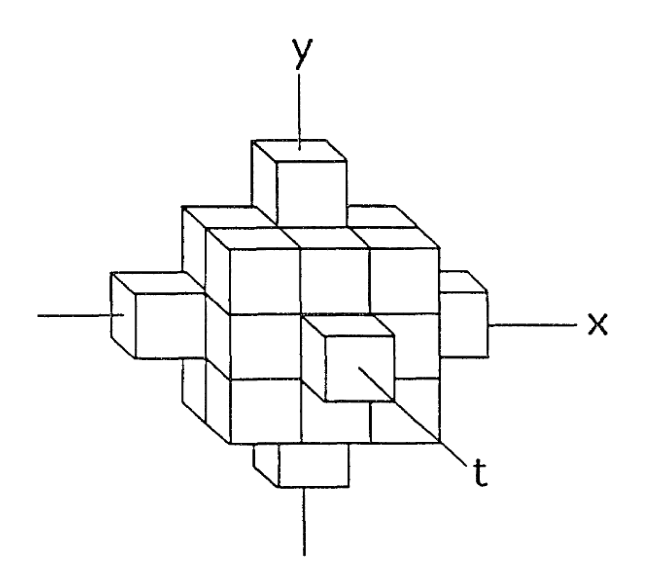
\includegraphics[width=0.3\textwidth]{images/20_neighbourhood.png}
\caption{20-cell, two step neighbourhood in space and time\cite{meyer1989learning}}
\label{fig:20-near}
\end{figure}

The fitness function used is
\begin{align}
                    F &= I - \frac{2^m}{N}\\
    \text{where\ }  I &= \sum P(s, s_1, ..., s_m)\log_2{\frac{P(s, s_1, ..., s_m)}{P(s)P(s_1, ..., s_m)}}
\end{align}

Here, $I$ is the mutual information of the subtemplate and represents the amount of information, measured in Shannon bits, that can be obtained about the value of the central cell from subtemplate states. It is calculated by summing across all $2^m$ configurations of the subtemplate in the data and across both values of $s \in \{0,1\}$. The second term in the fitness function ensures that subtemplates of varying sizes are treated appropriately by proportionately penalising large subtemplates that, by nature, will contain more information. $N=20$ is the size of the master template.\\

The genetic algorithm initialises the population at a randomly chosen subset of possible subtemplates. Selection is performed using a truncated linear ranking. Crossover is applied using an arbitrary cut in space-time on the master template as the crossover point. Point mutation is applied by either adding or removing a single cell from each candidate. This process is iterated to converge towards an optimum.\\

As the first notable exploration of learning CA properties with genetic algorithms, this paper demonstrates the ability of genetic algorithms to efficiently traverse an opaque search space. The algorithm precisely learns neighbourhoods interior to the master template such as the one time step Moore neighbourhood and even when the objective neighbourhood lies partially outside the master template, the algorithm successfully finds a close approximation. For example, when given data produced by a one time step von Neumann neighbourhood, the algorithm learns a neighbourhood set that produces correct behaviour 96\% of the time on tested targets.\\

This work also raises many questions for future research. The most pertinent is whether it is possible to link learned rules to existing and future theoretical models. Moreover, this work only explores binary state CA but application of similar techniques on continous-state CA could closer approximate the partial differential equations that underlie the physical processes being modelled.\\

Finally, this paper focuses on optimising the neighbourhood set of the CA model only. It aims to establish \textit{which} parameters in a local vicinity of a current cell are most relevant to predicting the future state, not \textit{how} those parameters are combined and transformed to produce the result.\\ In this thesis, we are interested in going beyond this and approximating the full transition function. In some cases we will fix the neighbourhood function used to reduce our search space under the assumption that techniques from this paper can be used to find optimal sub-neighbourhoods if they exist.\\


\subsection{Learning 1D Transition Functions}

There are a number of problems in elementary CA computation that have piqued academic interest from both analytical and computation angles. One example is the firing gun synchronisation problem\cite{moore1964firing} which seeks a rule that minimizes the time to get a CA from a quiescent state (all 0) to a firing state (all 1). Another is the density classification problem, or majority problem, which aims to find a binary elementary CA rule that accurately performs majority voting. That is, all cells converging to the state that dominates the initial condition. Despite their simple formulation, both of these problems require the transfer of information through compressed, latent representations and a global consensus based on localised computations. This makes them useful benchmarks when measuring the capability of CA and the algorithms used to design them. For the sake of brevity, we focus only on the majority problem in this section. We formalise it in Def~\ref{def:majority-problem}.

\begin{definition}[Majority Problem]\label{def:majority-problem}
An elementary CA of size N solves the majority problem for some initial conditions $\{\sigma_i\}_{i=1}^{N}$ if $\exists T$ s.t. $\forall t > T$:
\begin{equation}
    \sigma_i(t) = 
    \begin{cases}
    0, & \sum_{i=1}^{N}\sigma_i(0) < \frac{N}{2} \\
    1, & \sum_{i=1}^{N}\sigma_i(0) > \frac{N}{2}
    \end{cases}
\end{equation}
The desired result is undefined if the initial state contains an equal number of 0 and 1 cells.
\end{definition}

The Gacs-Kurdyumov-Levin (GKL) rule is a human-designed solution to solve this problem. The function, as defined in Def~\ref{def:gkl}, allows consensus to be reached in $O(N)$ time and, for $N=149$, achieves success on 81.6\% of inputs\cite{gacs1978one}. Modifications throughout the 1990s incrementally improved this classifier\cite{das1995evolving}. Although these were very promising, the human designed aspect of these algorithms meant there was little to support their optimality compared to others in the rulespace.

\begin{definition}[GKL Classifier] \label{def:gkl}
A GKL density classifier is an elementary CA on periodic boundary conditions with transition function
\begin{equation}
   \sigma_i(t+1) =
    \begin{cases}
    Mo(\sigma_{i-3}(t) + \sigma_{i-1}(t) + \sigma_i(t)), & \sigma_i(t) = 0 \\
    Mo(\sigma_i(t) + \sigma_{i+1}(t) + \sigma_{i+3}(t)), & \sigma_i(t) = 1
    \end{cases}
\end{equation}
where $Mo(.)$ returns the mode of its arguments.
\end{definition}

A seminal series of work by Mitchell, Crutchfield, and Das\cite{mitchell1996evolving} tackled this issue by automating the process of CA transition function design through evolutionary computation. These works made effective use of genetic algorithms operating on fixed length bitstrings. Rules with radius $r = 3$ were considered, leading to chromosomes of length $2^{2r+1}=128$. The size of the rulespace was therefore $2^{128}$ which eliminates the possibility of any exhaustive search. The size of the CA itself was $N=149$, chosen to be odd so that the solution to the majority problem is well defined. Upon initialisation, 100 chromosomes are chosen from a distribution that is uniform over chromosome density. This can be viewed as picking the binary representations of 100 samples from a binomial distribution. This is markedly distinct from the usual unbiased distribution which assigns each bit in the chromosome to 0 or 1 with probability 0.5, equivalent to picking 100 samples from the $Uniform(0, 128)$ distribution. The choice of binomial initialisation has been shown to considerably improve performance\cite{mitchell1994evolving}. At each generation, 100 new initial conditions (ICs) were created and fitness was defined as the percentage of correctly classified ICs. This stochastic fitness function was effective at reducing overfitting. A $(\mu+\lambda)$ selection method was employed with $\mu=20$ and $\lambda=80$ and mutation was performed with a two-point crossover. Although not as accurate as GKL, the best discovered solution still achieves a 76.9\% accuracy. However, the evolved solutions were not very sophisticated. Most fell into the category of "block-expanding algorithms" or simple "particle-based algorithms" shown in Figure~\ref{fig:1d-transitions} as (a) and (b) respectively. In the former case, white and black boundaries meet to form a vertical line whereas, in the latter, they form a checkerboard region to propagate signals about ambiguous regions across the CA.

\begin{figure}[H]
\centering
            \subfloat[Block-Based]{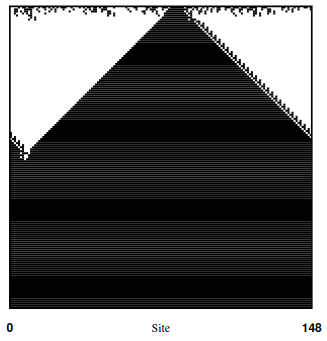
\includegraphics[height=.3\textwidth]{images/block-expand.png}}\hfill
            \subfloat[Particle-Based]{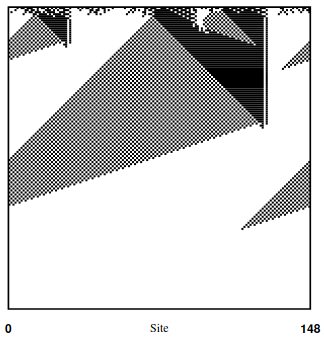
\includegraphics[height=.3\textwidth]{images/particle-based.png}}\hfill
            \subfloat[Koza Algorithm]{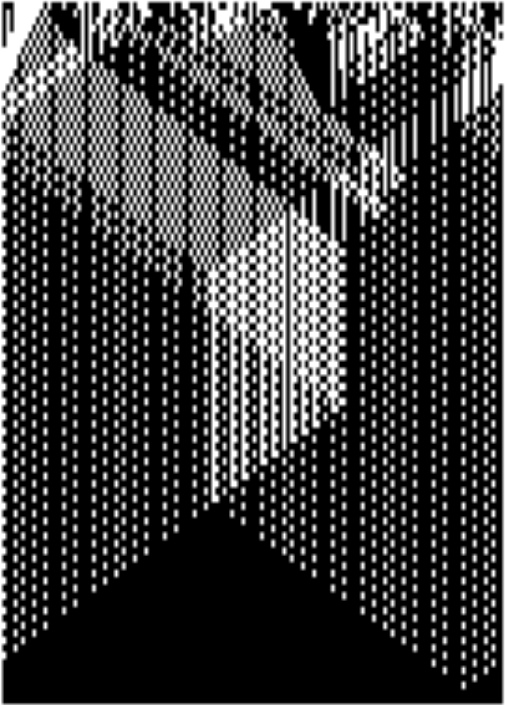
\includegraphics[height=.3\textwidth]{images/koza.png}}\hfill
            \caption{Space-time behaviour of discovered transition functions on randomly initialised elementary CA of size N=149. (a) and (b) by Mitchell et al.\cite{mitchell1996evolving} and (c) by Andre et al.\cite{andre1996discovery}}
\label{fig:1d-transitions}
\end{figure}

A later work by Andre, Bennett, and Koza\cite{andre1996discovery} uses genetic programming to achieve superior results qualitatively and quantitatively. The obtained solution uses various internal representations of density to transfer and collate information across the CA as showin in Figure~\ref{fig:1d-transitions} (c). It attains an accuracy of $\sim$82.3\%. However, with its numerous latent representations of density, it is more difficult to intuitively understand how the Koza algorithm works and what patterns it is capable of producing than it is to understand how the particle-based algorithm works. Recently, it was proven that a perfect density classification rule for an infinite CA in any dimension, stochastic or deterministic, is impossible\cite{buvsic2012density}. However, evolutionary computation still surprises in its ability to find approximations with ever-increasing performance. 

\subsection{Learning 2D Transition Functions}

Few attempts have been made to extend evolutionary algorithms to multidimensional CA. A key series of work by Breukelaar and B{\"a}ch\cite{breukelaar2004evolving} shows that genetic algorithms can effectively solve information transfer problems on 2D CA such as the majority problem, AND problem, and XOR problem. The AND and XOR problems, which we collectively call the logical problems, aim to set the state of every cell to the result of the respective logical operation on the initial state of the top left and bottom right cells. These logical operators are picked because the result cannot be calculated from a single operand alone. In other cases, like the OR operator, we can deduce that the result will be true from either of the operands being true. For the majority problem, tests showed that results with a fitness of up to 70\% have been acheived evolved using a von Neumann neighbourhood. For the logical problems, a von Neumann neighbourhood can elicit results with over 90\% accuracy and a Moore neighbourhood with perfect accuracy. Notably, it was shown that crossover did little to aid the evolution process in the logical problems and frequently even hindered progress.\\

They also show promise at small scale morphogenesis. Morphogenesis for CA is the problem of evolving a rule that, given an initial condition, produces a particular goal state within a certain number of steps. In this work, the goal bitmaps were 5x5 square patterns shown in Figure~\ref{fig:goal-bitmaps}.\\

\begin{figure}[H]
\centering

\includegraphics[width=.5\textwidth]{images/bitmap-goals.png}
\caption{Goal bitmaps for morphogenesis experiment\cite{breukelaar2004evolving}}
\label{fig:goal-bitmaps}
\end{figure}

Using only mutation, not crossover, the algorithm was able to find a rule to produce every goal bitmap from a seed state of a single live cell in the centre of the CA within 5000 generations as shown in Figure~\ref{fig:xor}. This is very promising and indicates that the value of genetic algorithms in producing CA rules not only encode information transfer mechanisms, but latent representations of data itself.\\

\begin{figure}[!h]
\centering
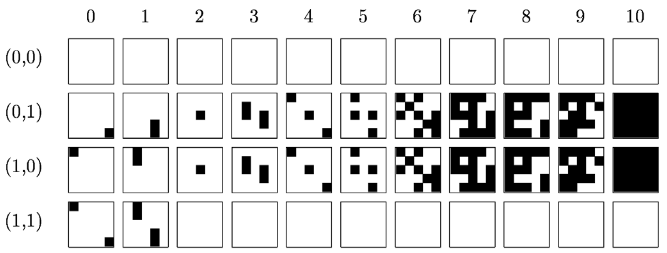
\includegraphics[width=.8\textwidth]{images/XOR-ca.png}
\caption{Iterations of XOR CA for 4 possible input states\cite{breukelaar2004evolving}}
\label{fig:xor}
\end{figure}

Early work by Wulff and Hertz in 1992\cite{wulff1992learning} uses a lattice-shaped neural network style structure to learn CA dynamics. Each node in this lattice is a Probabilistic Logic Node, also known as a $\Sigma-\Pi$ unit \cite{gurney1992training}. These units are capable of representing any boolean function. That is to say $ \forall f: \mathbb{R}^N \to \{-1, 1\}, \exists~w_1, w_2, ... , w_N \in \R $ such that,

\begin{equation} \label{eq:sigma_pi}
f(S_1, S_2, ..., S_N) = sgn\left[ \sum_{j=1}^{N} w_j \prod_{i \in I_j} S_i(t) \right]
\end{equation}

where index set $I_j$ is randomly drawn from the integers $\{1, 2, ..., N\}$ without replacement. Notably, these units do not require input from every neighbour to learn successfully. In fact, this paper found any index set of size $|I_j| \geq \frac{N}{2}$ to be sufficient. This insight significantly reduced training time. Three learning goals were established for the network. In order of increasing difficulty they were:

\begin{enumerate}
  \item Extrapolation: Learn to simulate a CA for a \textit{particular} initial condition at any time
  \item Dynamics : Learn to simulate a CA for \textit{any} initial condition after short-lived patterns have been exhausted
  \item Full Rule : Learn to simulate a CA for any initial condition at any time
\end{enumerate}

This work was largely concerned with class 3 (chaotic) and class 4 (complex) behaviour.  All 9 known examples of class 3 1D CA were tested on. However, at the time, it was believed that 1D CA could not exhibit class 4 behaviour. Therefore, testing was also conducted on Conway's Game of Life. With a shared network across all cells, this approach was very promising, with extrapolation and dynamics being very easy in the 1D and 2D cases. Learning the full rule was much harder. The network only was able to do so for 4 out of the 9 candidates in the 1D case. This work also divided class 3 elementary CA into two categories according to how easy it is to learn their underlying rule. However, this work was limited to only exploring class 3 and class 4 CA.\\

More recent work has used modern feed-forward neural networks to learn transition functions for morphogenesis. Specifically, in \textit{Growing Neural Cellular Automata, (Mordvintsev et al., 2020)}\cite{mordvintsev2020growing}, a CA is designed with a transition function that is itself a forward pass of a trainable convolutional neural network. In this form, the CA is trained to converge to complex yet stable image patterns from a single seed as shown in Figure~\ref{fig:nca}. Later works build upon these techniques to learn full dynamical systems such as the Boids algorithm\cite{grattarola2021learning}. However, even for small neural networks, the potential rulespace is enormous with thousands of possible parameters. Ultimately, this makes a deep learning derived solution powerful yet intractable. Although CA with neural network transition functions are much more expressive and powerful due to the granularity with which behaviour can be tuned, they arguably defeat the purpose of encoding rich behaviour in a compressed chromosome such as a bitstring.\\

\begin{figure}[!h]
\centering
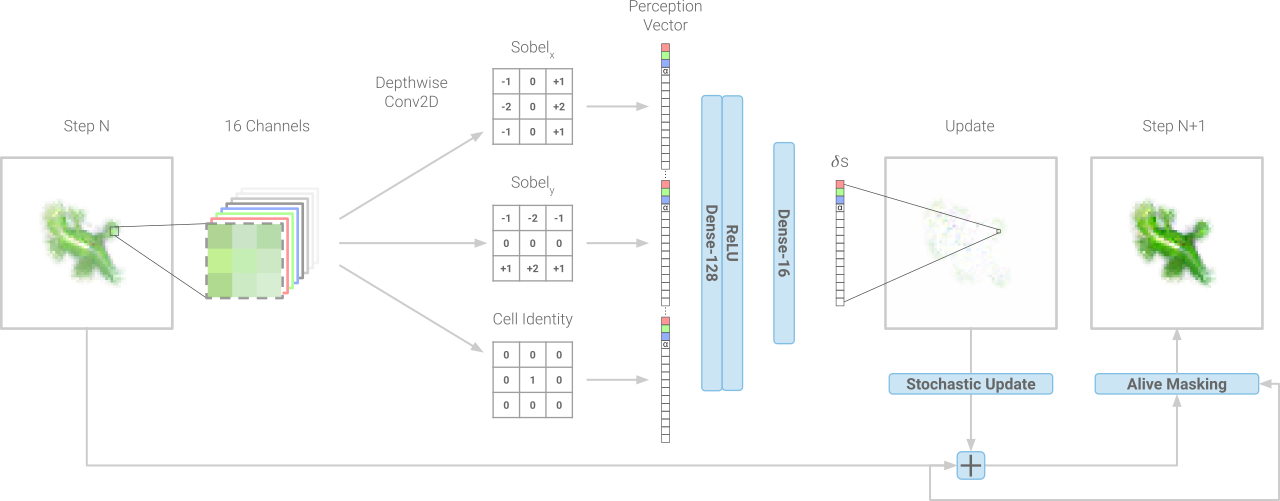
\includegraphics[width=\textwidth]{images/nca.png}
\caption{Single training step for a neural cellular automaton\cite{mordvintsev2020growing}}
\label{fig:nca}
\end{figure}

At the time of writing, no attempts have been made to use evolutionary computation to learn full rule dynamics of life-like cellular automata. This thesis is a first attempt.

\section{Gray-Scott Systems: Exploration} \label{sec: gs-exploration}

Pearson\cite{pearson1993complex} classifies patterns arising from Gray-Scott models into 12 categories  based on temporal factors such as stability and decay rate as well as spatial factors such as regularity and emergence of subpatterns like spots and stripes. These are shown in Figure~\ref{fig:pearsons}. Each simulation operates on a $256 \times 256$ grid with periodic boundary conditions. The initial conditions are uniform ($u = 1$, $v = 0$) with the exception of a $20 \times 20$ square patch in the centre with ($u=\frac{1}{2}$, $v=\frac{1}{4}$) perturbed with $\pm 1\%$ Gaussian noise.\\

\begin{figure}[!h]
\centering
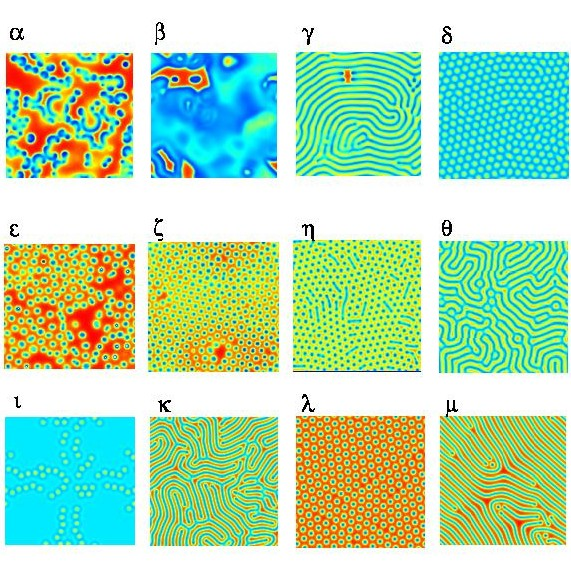
\includegraphics[width=.8\textwidth]{images/pearsons.jpg}
\caption{Pearson's 12 categories of Gray-Scott systems\cite{pearson1993complex}}
\label{fig:pearsons}
\end{figure}

Pearson discovered a threshold near which interesting behaviour can be observed. As the parameters $f$ and $k$ move across the threshold, the system transitions from one uniform stable state to another. These uniform states are dubbed $R$ for red and $B$ for blue. The red state corresponds to the trivial fixed point ($u = 1$, $v = 0$) and the blue state depends on the exact parameters, but tends to exist around ($u = 0.3$, $v = 0.25$). During the transition between these states, the system has two equilibria and at least one of these is a saddle point. The change in stability and number of equilibria elicits Turing instability and causes the aforementioned patterns to emerge. This unstable region is depicted in Figure~\ref{fig:pearsons-threshold} between the dotted and solid lines. Considering a fixed kill rate, the system transitions from blue to red as f increases at the upper solid line through saddle-node bifurcation wherein the two equilibria collide and annihilate. This explains why the transition is so sudden in this region. As f decreases through the dotted line, Hopf bifurcation occurs and a branch of periodic solutions is formed. These create a larger region of interesting behaviour.
\pagebreak

\begin{figure}[!h]
\centering
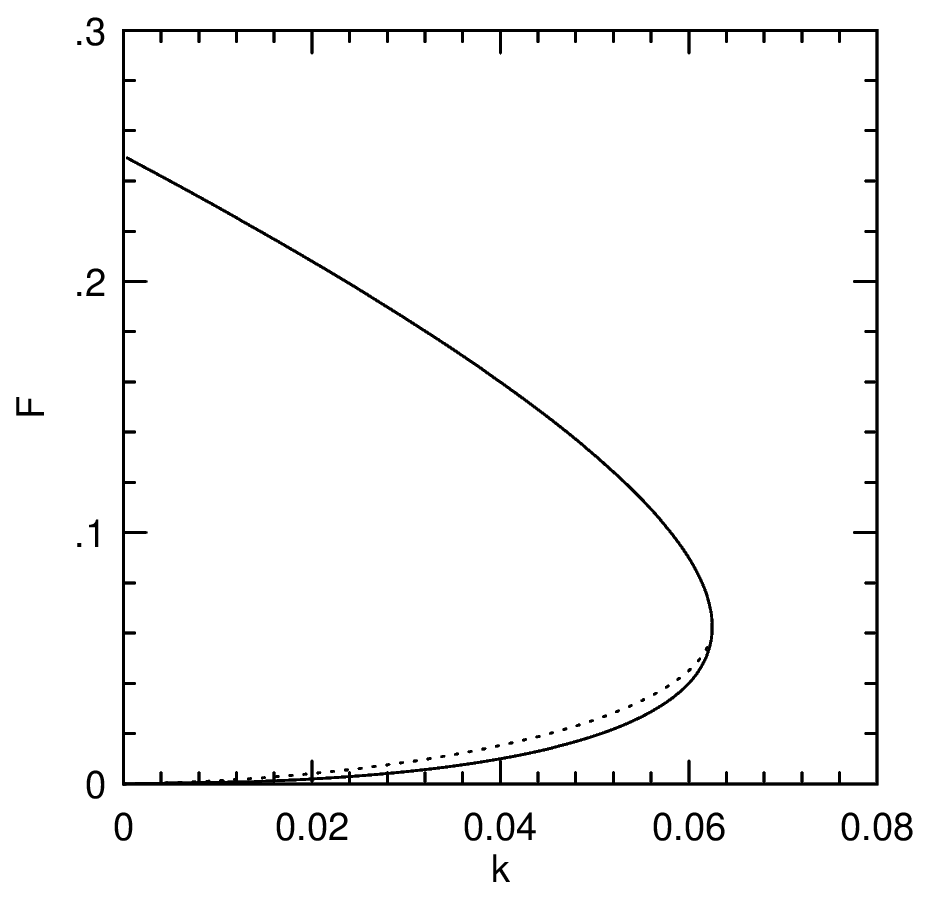
\includegraphics[width=.5\textwidth]{images/pearson-threshold.png}
\caption{Phase diagram of Gray-Scott systems\cite{pearson1993complex}}
\label{fig:pearsons-threshold}
\end{figure}

However, Pearson's analysis is limited by the initial condition he uses. Contrarily, Munafo\cite{munafo2014stable} is able to reveal 5 new types of pattern differentiated from others by oscillation and spot shape by using a single central patch of ($u = 0$, $v=1$) on an otherwise red background (i.e. an inversion of Pearson's initial condition) or several spots of diverse ($f$, $k$) values. One example is the $\rho$ pattern shown in Figure~\ref{fig:munafo-rho}. In imprecise terms, the feed rate controls oscillation, stability, and chaos while the kill rate controls the shape and quality of objects formed.

\begin{figure}[H]
\centering
            \hfill
            \subfloat[f = 0.090, k = 0.059]{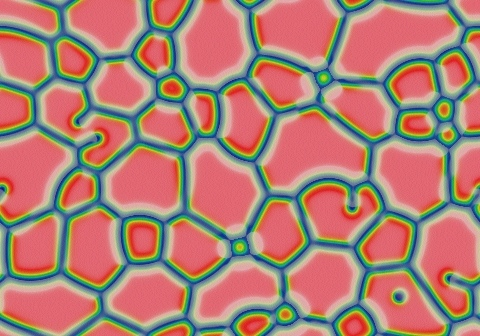
\includegraphics[width=.3\textwidth]{images/munafo-rho-1.jpg}}\hfill
            \subfloat[f = 0.102, k= 0.055]{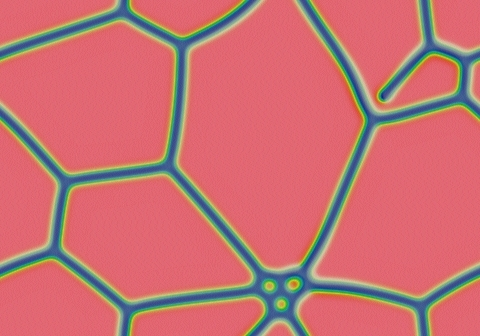
\includegraphics[width=.3\textwidth]{images/munafo-rho-2.jpg}}
            \hfill
            \hfill
            \caption{The $\rho$ class of Gray-Scott pattern resembles a set of soap bubbles under surface tension. These clearly do not resemble any of the 12 Pearson categories. \cite{munafo}}
\label{fig:munafo-rho}
\end{figure}

Munafo also presents a mapping from the Pearson / Munafo classes to the universal complexity classes established by Wolfram. However, due to the clear variety of behaviour in continuous state systems, three additional subclasses are presented.
\begin{itemize}
    \item Class 2-a: These combine features of class 1 and 2. Certain starting conditions look like class 2 but eventually induce cascades which lead to asymptotic stasis as shown in Figure~\ref{fig:munafo-2}.
    \item Class 3-a: A subset of class 3. Although the patterns formed are relatively homogenous after a certain period like all class 3 systems, these patterns do not exhibit unending chaos. Instead, there are areas of long-lived localized stability through which chaos propagates as shown in Figure~\ref{fig:munafo-3}. However, these are not class 2 or 4 as the rate of change approaches a non-zero constant.
    \item Class 4-a: These are hypothetical class 4 systems that are subject to the halting problem. No example has yet been proven.
\end{itemize}

\begin{figure}[!h]
\captionsetup[subfigure]{labelformat=empty}
\centering
            \subfloat{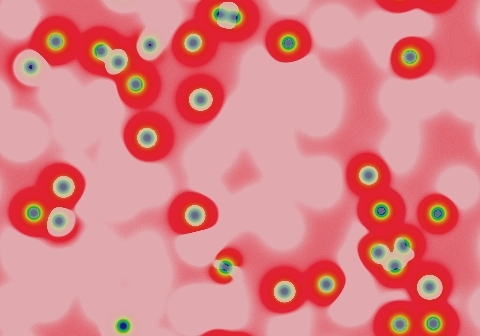
\includegraphics[width=.3\textwidth]{images/munafo/2/1.jpg}}\hfill
            \subfloat[f = 0.046, k = 0.067]{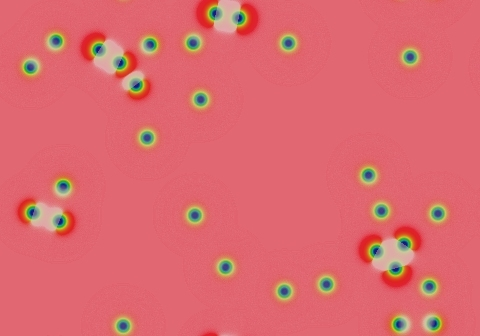
\includegraphics[width=.3\textwidth]{images/munafo/2/2.jpg}}\hfill
            \subfloat{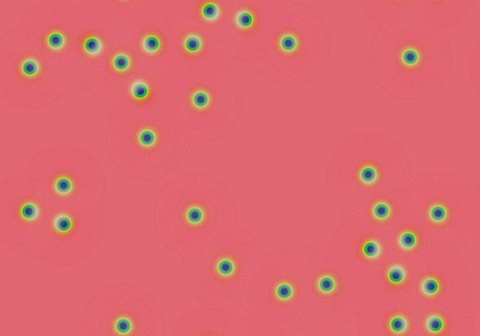
\includegraphics[width=.3\textwidth]{images/munafo/2/3.jpg}}\hfill
            \newline
            \subfloat{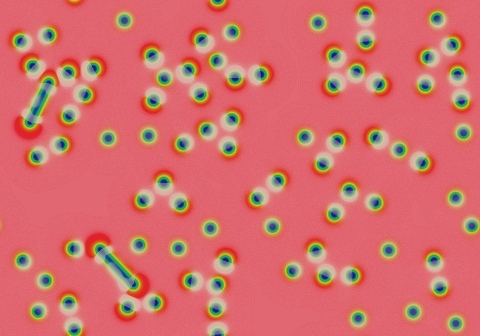
\includegraphics[width=.3\textwidth]{images/munafo/2a/1.jpg}}\hfill
            \subfloat[f = 0.066, k = 0.065]{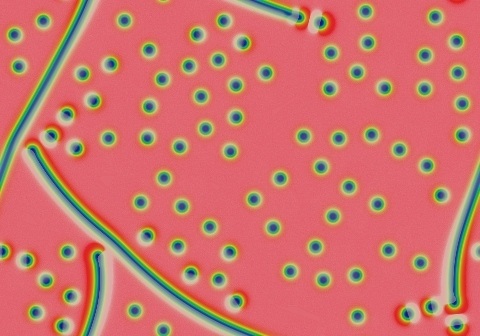
\includegraphics[width=.3\textwidth]{images/munafo/2a/2.jpg}}\hfill
            \subfloat{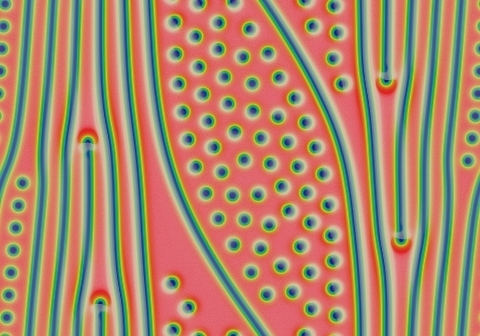
\includegraphics[width=.3\textwidth]{images/munafo/2a/3.jpg}}\hfill
            \caption{Class 2 behaviour (top) against class 2-a behaviour (bottom). Time moves left to right. \cite{munafo}}
\label{fig:munafo-2}
\end{figure}

\begin{figure}[!h]
\captionsetup[subfigure]{labelformat=empty}
\centering
            \subfloat{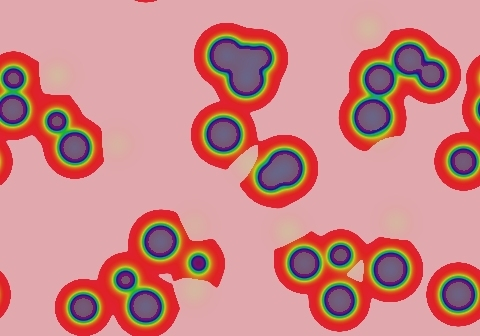
\includegraphics[width=.3\textwidth]{images/munafo/3/1.jpg}}\hfill
            \subfloat[f = 0.014, k = 0.049]{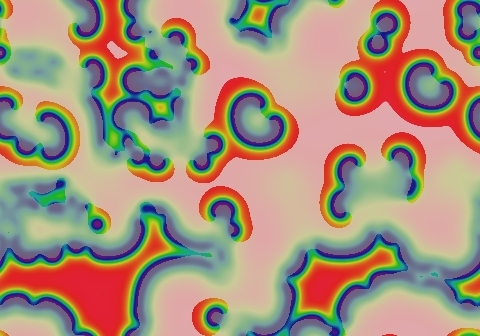
\includegraphics[width=.3\textwidth]{images/munafo/3/2.jpg}}\hfill
            \subfloat{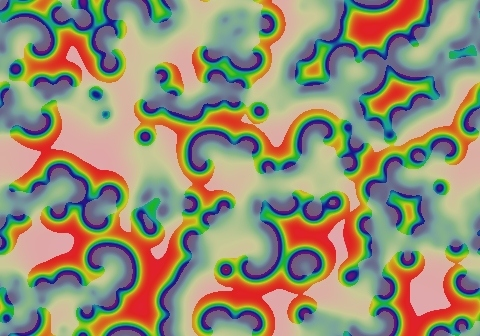
\includegraphics[width=.3\textwidth]{images/munafo/3/3.jpg}}\hfill
            \newline
            \subfloat{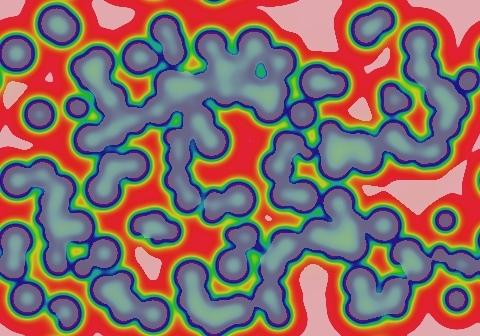
\includegraphics[width=.3\textwidth]{images/munafo/3a/1.jpg}}\hfill
            \subfloat[f = 0.022, k = 0.053]{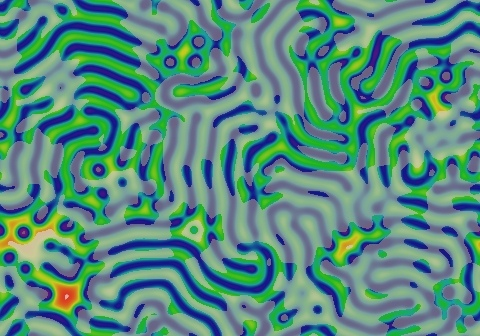
\includegraphics[width=.3\textwidth]{images/munafo/3a/2.jpg}}\hfill
            \subfloat{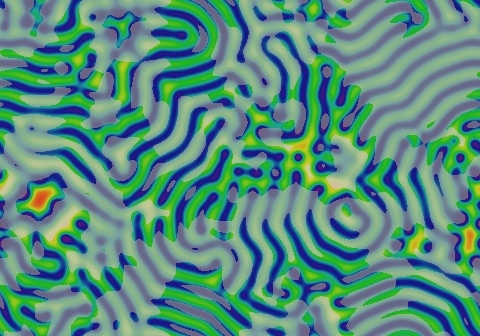
\includegraphics[width=.3\textwidth]{images/munafo/3a/3.jpg}}\hfill
            \caption{Class 3 behaviour (top) against class 3-a behaviour (bottom). Time moves left to right. \cite{munafo}}
\label{fig:munafo-3}
\end{figure}

One parameterisation of particular interest is ($f=0.0620$, $k=0.0609$). Under this setting, certain patterns can be observed that move indefinitely until intercepted. These U-shaped patterns called \textit{skates} closely resemble the gliders in Conway's Game of Life and open the door to questions of universal computation.\\

Finally, Figure~\ref{fig:xmorphia} shows a schematic map of the ($f$, $k$) parameter space with the complex, crescent-shaped region showing the variety of patterns that can exist.

\begin{figure}[!h]
\centering
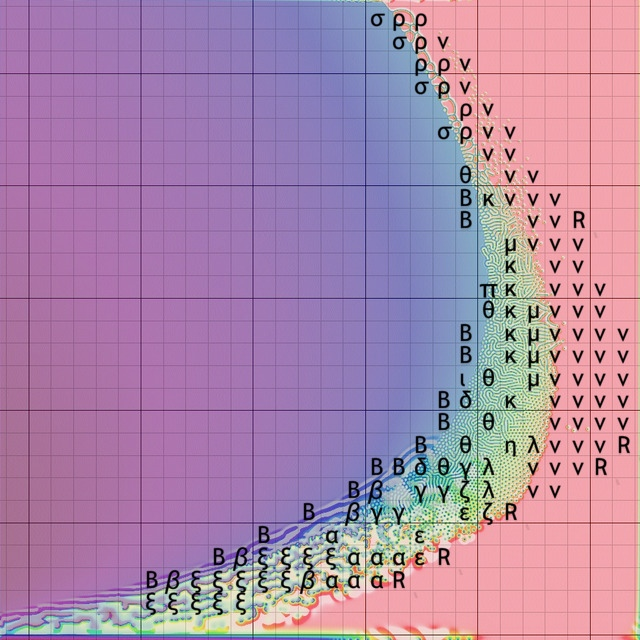
\includegraphics[width=.9\textwidth]{images/munafo/xmorphia.jpg}
\caption{Map of Gray-Scott parameter space depicting all 19 Pearson-Munafo classes \cite{xmorphia}}
\label{fig:xmorphia}
\end{figure}

\section{Gray-Scott Systems: Learning}

As a system of partial differential equations, Gray-Scott systems are typically solved using numerical analysis such as finite difference methods\cite{manaa2013successive}. There are not many attempts learn solutions using machine learning, possibly due to the success of state-of-the-art numerical methods at solving such systems.\\

One key work that does use machine learning is \textit{Physics-Informed Neural Networks Approach for 1D and 2D Gray-Scott Systems (Giampaolo et al., 2022)}\cite{giampaolo2022physics} as shown in Figure~\ref{fig:paulo}. Finite difference methods are used to produce a constrained search space of physically feasible solutions for a neural network to learn on. In particular, physics-informed neural networks (PINNs) use a residual loss that encodes the divergence of a solution from the physical laws underlying the problem. The network aims to become a surrogate model of the true system and can be trained in a forward or inverse setting. In this work, at each of $n$ time points, forward difference methods are used to obtain the correct "known" state which is fed into the surrogate model. This is to avoid the system converging to local minima under extended simulation times. Without corrections based on known data, the final Gray-Scott system exhibits trivial state in which the reactant either disperses entirely or overwhelms the domain. The loss function depends on the differential equation, the initial conditions and the known data.\\

The ANN architecture consists of 4 hidden layers of 20 neurons each with a $\mathit{tanh}$ activation on input and $\mathit{sigmoid}$ activation on output. The initial and boundary conditions are of the same form as Pearson's analysis and 10 known data collections are performed at 500 time step intervals. When testing on 4 common parameterisations, the system can mimic the patterns produced reasonably effectively with RMSE values between 0.1 and 0.3. As with many deep learning approaches, this method is computationally intensive with execution times of about 15 minutes on a GPU NVIDIA GeForce RTX 3080 with CPU intelcore i9-9900k and 128 GB of RAM. However, PINNs possess better ability to generalise compared to "blind" neural networks, due to the physical constraints imposed in the loss function.

\begin{figure}[!h]
\centering
\subfloat[Mitosis pattern (f = 0.028, k = 0.062)]{
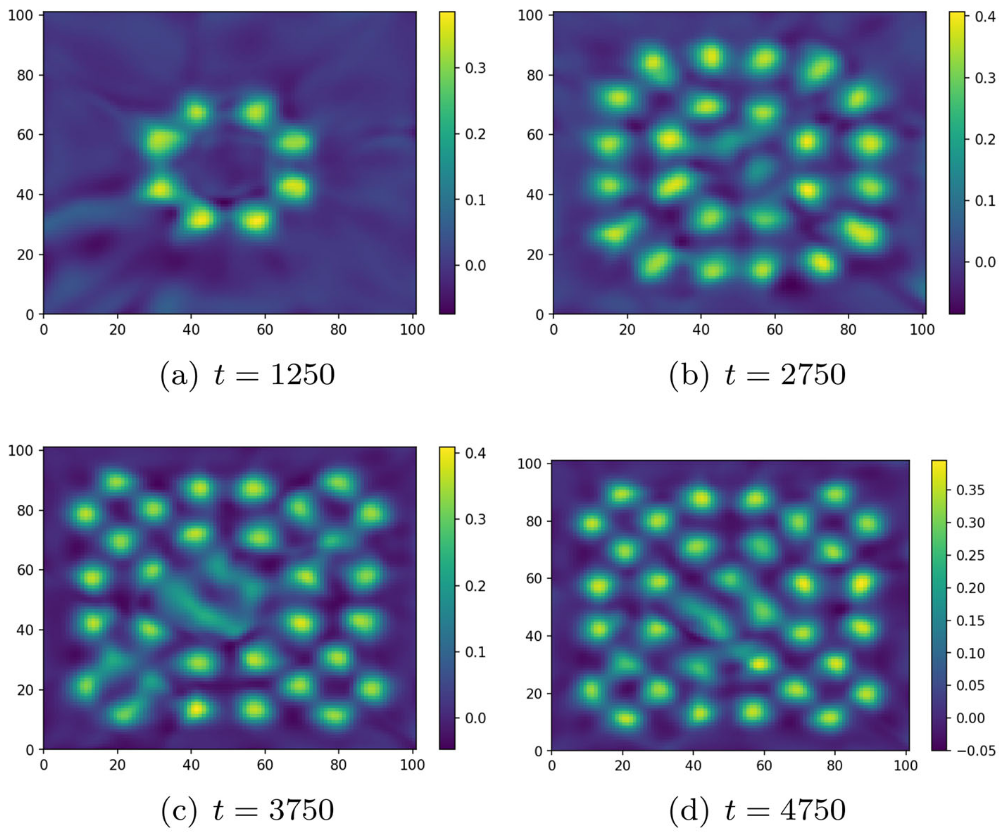
\includegraphics[width=.45\textwidth]{images/paulo-mitosis.png}
}\hfill
\subfloat[Soliton pattern (f = 0.030, k = 0.060)]{
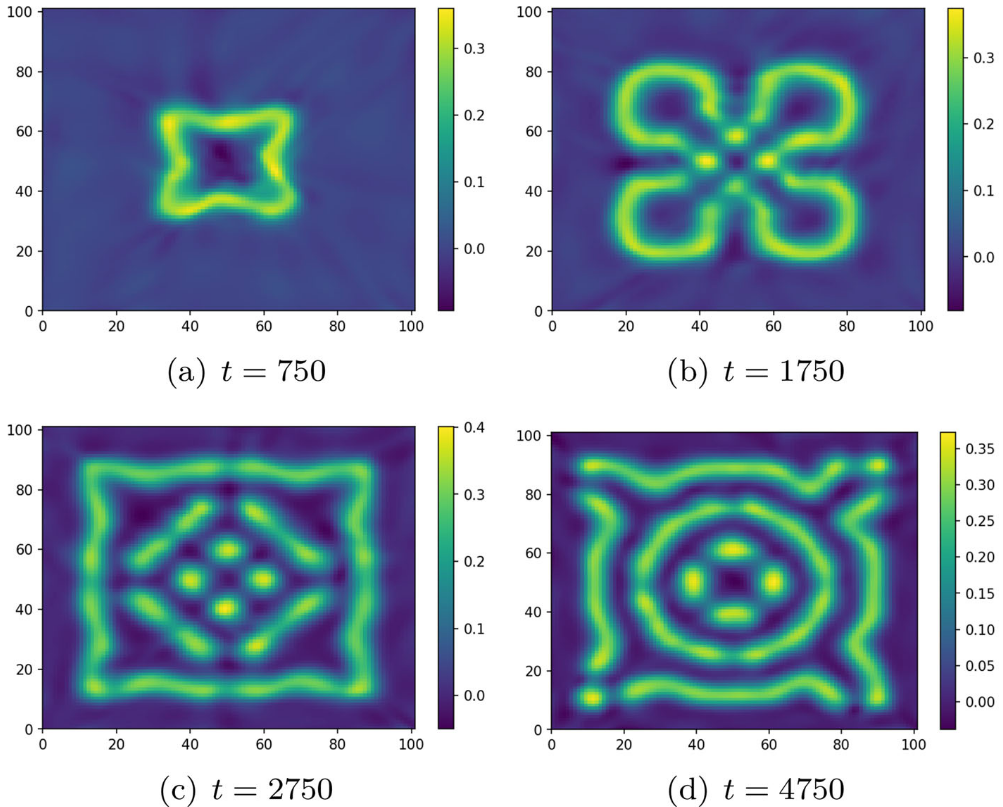
\includegraphics[width=.45\textwidth]{images/paulo-soliton.png}
}\hfill
\caption{Patterns predicted using PINN \cite{giampaolo2022physics}}
\label{fig:paulo}
\end{figure}